% Created 2010-08-27 Fri 20:48
\documentclass{article}


\title{Diameter of Random Clusters}
\author{Don Blair}
\date{27 August 2010}

\begin{document}



\setcounter{tocdepth}{5}
\tableofcontents
\vspace*{1cm}
\section{Introduction}
\label{sec-1}
\subsection{General overview}
\label{sec-1.1}

The Potts Model has been employed in an impressive number contexts, both in and oustide physics. [REF] Via the F-K mapping of the Potts Model onto the Random Cluster model [REF], the $q=1$ Potts model is known to be equivalent to the Percolation Model, while the $1=2$ Potts model is equivalent to the Ising Model.
$q>2$ versions of the Potts model also have important applications [REF]. In all of these contexts, it is of interest to study the behavior of the clusters of Potts spins that arise in the model -- their typical size, shape, and phase behavior.  A well-studied [REF]
geometric property of Potts clusters is the average \emph{chemical distance} on the cluster -- defined as the shortest path along satisfied bonds between two arbitrarily-chosen spins on the cluster.  
In this paper we introduce and study the behavior of a new geometric property of Potts clusters: the cluster \emph{diameter}, defined as the longest shortest path between any two sites on a cluster.  The diameter of a cluster places a limit on the maximal rate at which processes can spread to all sites a cluster; knowing how the typical diameter of a random cluster scales with system size, $L$, should prove useful in assessing, for example, the efficiency of algorithms defined on such clusters [REF]. 
We report on numerical studies that reveal the scaling of the diameter of the largest cluster in the lattice for Potts Models with $q=1,2,3,4$ on the 2D square lattice, $q=1,2,3$ on the 3D cubic lattice, and $q=1,2$ on the 4D hypercubic lattice.
\subsection{History: Chemical distance}
\label{sec-1.2}

The scaling exponent $d_{min}$ for the chemical distance has been studied extensively for the Percolation Model (Potts Model with $q=1$) [REFS], using various methods [REFS].  
This focus on the chemical distance arose out of the usefulness of this quantity in assessing the spread of processes within porous media -- e.g., oil in rock, or water in a gel -- that are well-described by the Percolation Model. The chemical distance provides an indication of how ``direct'' or ``torturous'' the most likely path between various points in a given media will be. In the graph theory context, the chemical distance can be thought of simply as the shortest path between two vertices on a connected graph.
\subsubsection{Previous results}
\label{sec-1.2.1}
\paragraph{q=1}
\label{sec-1.2.1.1}

To date, the most accurate reported value for the average chemical distance in Potts $q=1$ (Percolation) clusters on the square lattice is 1.13086 [?] [REF].  For $q=1$ in 3D, 4D, and 5D, the best known values are those reported by [REF? Stanley et. al?].  
\paragraph{q=2, greater}
\label{sec-1.2.1.2}

For Potts $q=2$ (Ising) Models, the best known value for the chemical distance are those reported by [??] in 2D, and by [??] for 3D cubic lattices.
\paragraph{Theory}
\label{sec-1.2.1.3}

Attempts to relate $d_{min}$ to other, known exponents -- have so far proven inconclusive.  Recently, Fink provided an exact relationship between $g_1$ [??] and [??], but this does not fix a value of $d_{min}$. 
\subsection{History: Diameter}
\label{sec-1.3}

In contrast, the \emph{diameter} of a connected graph is the distance between the two vertices which are furthest away from eachother (where here distance is defined as the shortest path along graph edges).   The diameter is commonly used as a parameter in assessing the efficiency of algorithms defined on connected graphs [REFS], and has been extensively studied on random graphs [REFS].
\subsubsection{Diameter in physical processes}
\label{sec-1.3.1}

The diameter is also of interest in physical systems, since correlations and transport processes that occur along bonds or connected paths in a cluster will be limited by the diameter of the cluster.  
\subsubsection{Diameter in Potts Model / Random Cluster Model}
\label{sec-1.3.2}

In particular, recent applications of the Potts Model in biophysics [REFS] display dynamics that are strongly dependent upon the diameter of the underlying clusters.
\subsubsection{Previous Results}
\label{sec-1.3.3}
\paragraph{Mean field theory results for random graphs}
\label{sec-1.3.3.1}

Because of its utility in computer science and mathematics, the diameter of certain types of graphs has been extensively studied [REFS].  The diameter of random graphs is known to scale as 
while the diameter of [insert another type of graph] behaves as [insert behavior].  For a review of the diameter of random graphs, see [REF].  The behavior of the diameter on Potts Model clusters has so far remained unexplored, so far as we are aware.  Because the random graph is considered to correspond to the infinite dimensional case of graphs on a lattice, theoretical results for the diameter of random graphs should match that of the diameter in critical 4D $q=4$ Potts model clusters.  

\begin{figure}[htbp]
\includegraphics[width=8cm]{fig2}
\caption[]{\label{fig:fig2} Illustration of a chemical distance (green) and diameter (red) on a typical Potts cluster configuration.}
\end{figure}
\section{Methods and Results}
\label{sec-2}

We study the scaling of both the chemical distance and the diameter of critical Potts Model clusters.  For $q=1$ in 2D, 3D, and 4D, we can compare our values for the chemical distance to those available in the literature.  Further, we can see how the scaling exponents for the chemical distance ($d_{min}$) and for the diameter ($d_{D}$) are related. 
\subsection{Simulation setup}
\label{sec-2.1}
\subsubsection{Used Swed-Wang algorithm (description?)}
\label{sec-2.1.1}

When simulating the Potts Model at criticality, it is useful to avoid critical slowing by means of a cluster flipping algorithm [REF]. We chose to employ the Swedsen-Wang [REF] algorithm, which works by 
\subsubsection{Spins stored in linear array, with mapping onto nearest neighbors for periodicity}
\label{sec-2.1.2}

A one dimensional array was used to store Potts spins; an additional one-dimensional array was used to enforce periodic boundary conditions by mapping spins onto their nearest neighbors.  
\subsubsection{Cluster identification using 'leath growth' method}
\label{sec-2.1.3}

Clusters were identified in the Swendsen Wang algorithm using an ``ant'' method [REF], which involves doing a (DEPTH? BREADTH?) - first search from all lattice sites along satisfied bonds.
\subsubsection{Measuring the chemical distance (review of literature)}
\label{sec-2.1.4}

We measured the chemical distance in a way that differs from typical methods found in the literature [REFS], but which appears to yield similar results (within [CITE ERROR BAR]).  We pick a site on the cluster at random, and perform a [DEPTH-FIRST? BREADTH-FIRST?] search along cluster bonds until all sites in the clusters have been visited.  The ``shell'' of the last site visited in this process is then equal to the length of the chemical path between the first site picked and the final site.  It is expected that this path will scale in the same way as does the chemical path, with $r \propto l^{d_{min}}$. In order to confirm this, we also measured the chemical distance by picking two arbitrary sites on the cluster and performing a breadth-first search from one of them until the other was reached, using the final chemical shell achieved in this manner as the value for the length of the chemical path between them; this resulted in values for the average chemical distance that were within \$.01\%\$. It is also reasonable to assume that we can replace $r$ with the system size $L$; we therefore measure the scaling of $d_{min}$ with $L$. 
\subsubsection{Measuring the diameter}
\label{sec-2.1.5}

In order to measure the diameter, we performed a Leath growth from all sites on the cluster; the largest chemical shell reached across all such Leath scans is equal to the length of the longest shortest path between any two cluster sites, or the diameter of the cluster.  For a cluster of $n$ connected sites, this method requires of order $n^3$ steps, and the associated CPU time becomes prohibitive for 2D lattices with sizes greater than $L=128$, or 3D lattices larger than $L=10$. For larger systems we therefore rely on the observed similarity between the chemical distance and the diameter, and use our measurement of the chemical distance -- an order $n$ process -- in lieu of the diameter.
\subsubsection{Thermalization and measurement intervals}
\label{sec-2.1.6}

In order to ensure that our measurements are uncorrelated, we made measurements of the chemical distance and diameter at intervals of app oximately $3*t_{corr}$. $t_{corr}$ is measured in units of sweeps, where one sweep is defined as [HOW IS ONE SW SWEEP DEFINED?]. For $q>1$ we allowed the system to thermalize for $X t_{corr}$ SW sweeps. Accordingly, $t_{corr}$ was measured for each
value of $q$ and system size $L$.  
\subsubsection{CPU time taken was X}
\label{sec-2.1.7}

Using the above methods, we estimated that the CPU time taken to simulate the 2D, q=1 Potts Model was $f(L)$ seconds, where $L$ is the lattice size.
\subsubsection{Measured for a range of L}
\label{sec-2.1.8}

For 2D, we measured $L=16,32,...FULL RANGE$ for each value of $q$; for the 3D system, we measured $L=FULL RANGE$. We needed to restrict our measurements to the chemical distance for 3D and 4D, as a measurement of the exact diameter became computationally prohibitive for large 3D and 4D systems.
\subsection{Analysis}
\label{sec-2.2}
\subsubsection{Linear fit to log(d) vs. log(L) plot, using ansatz.}
\label{sec-2.2.1}
\subsubsection{Other methods?}
\label{sec-2.2.2}
\subsubsection{for q=4, also tried log corrections.}
\label{sec-2.2.3}
\subsection{Results}
\label{sec-2.3}
\subsubsection{2D Results}
\label{sec-2.3.1}
\paragraph{q=1}
\label{sec-2.3.1.1}



\begin{figure}[htbp]
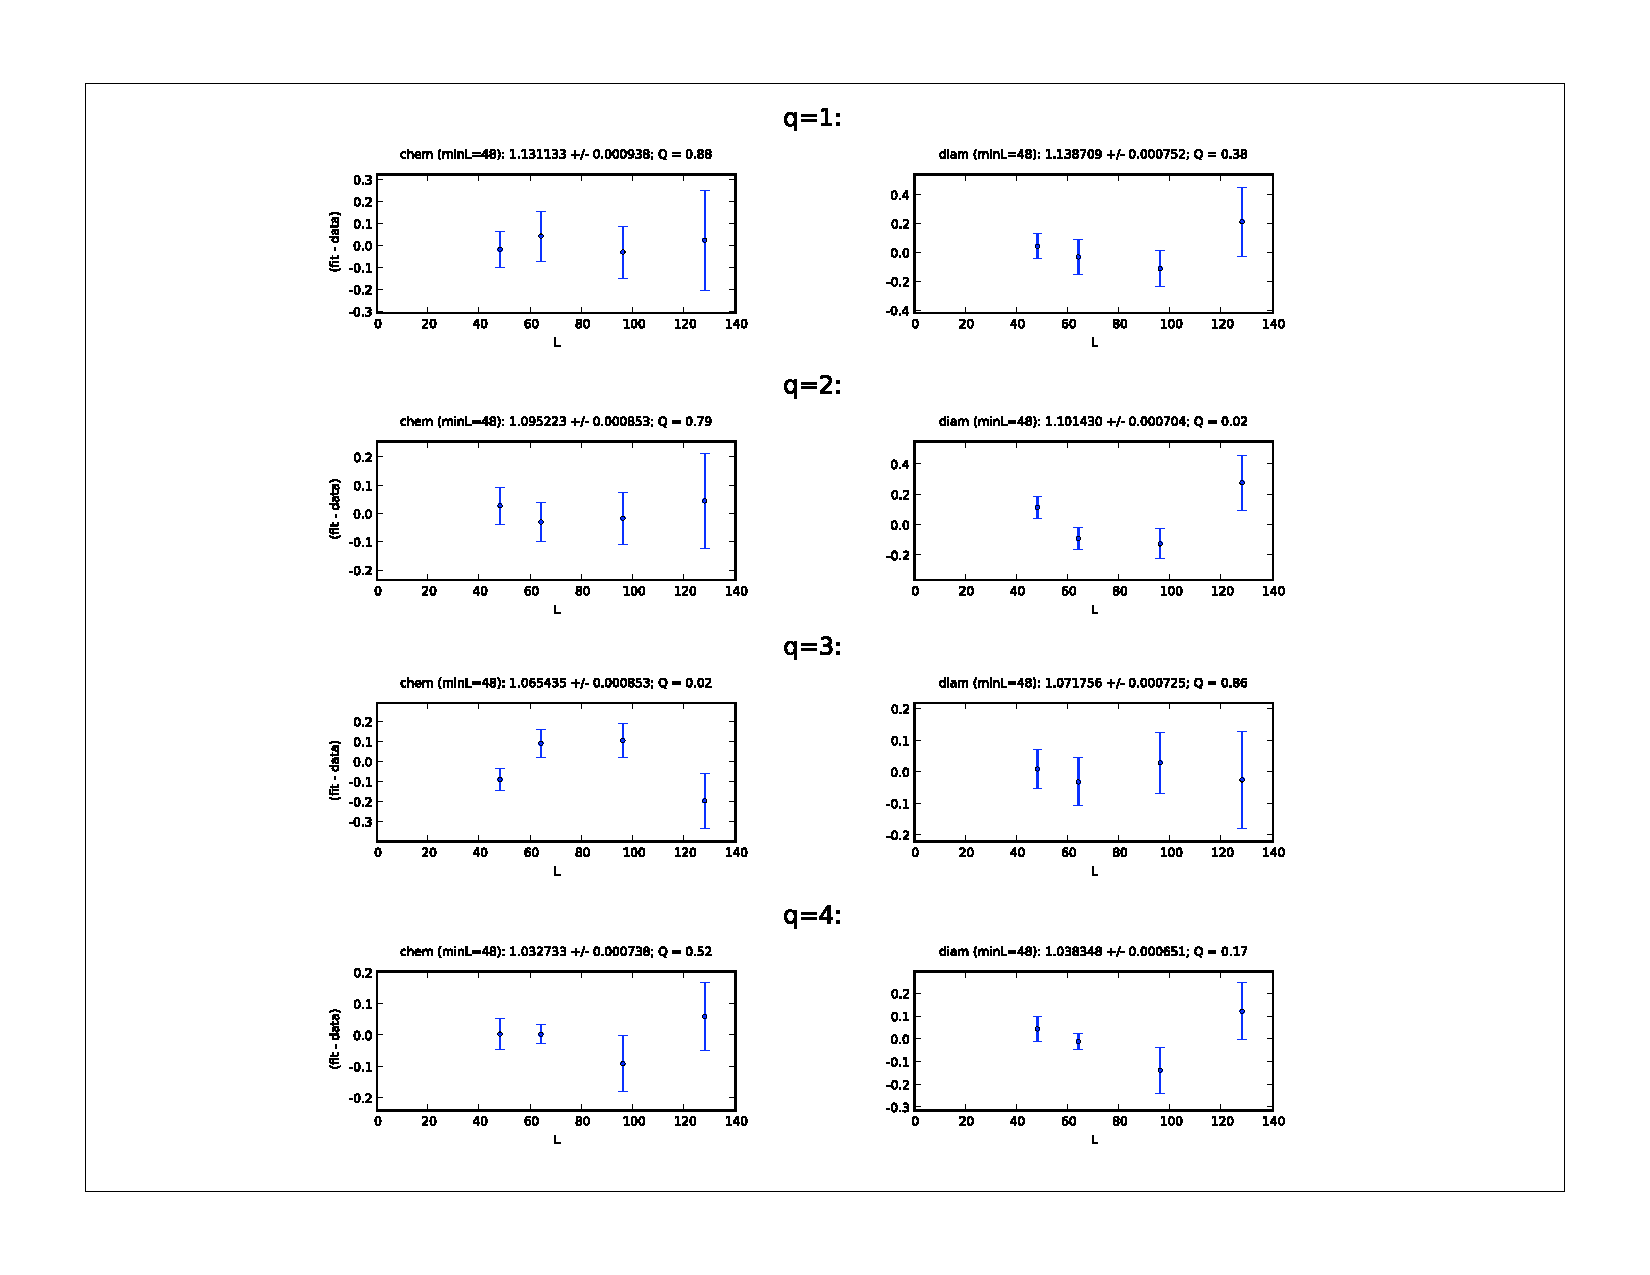
\includegraphics[width=16cm]{fig1}
\caption[]{\label{fig:fig1} 2D Potts Model: Difference between fit and data for the scaling of $d_{min}$ and $d_{diam}$.}
\end{figure}




\begin{itemize}
\item Correlation time was X.
\item Comparison of chem distance with literature.
\item Comparison of chem distance with diameter (very close).
\item FIGURE
\end{itemize}
\paragraph{q=2}
\label{sec-2.3.1.2}

\begin{itemize}
\item Correlation time was X.
\item Comparison of chem distance with literature.
\item Comparison of diameter with chemical distance.
\item FIGURE
\end{itemize}
\paragraph{q=3}
\label{sec-2.3.1.3}

\begin{itemize}
\item Correlation time was X.
\item Comparison of chem distance with literature.
\item Comparison of diameter with chemical distance.
\item FIGURE
\end{itemize}
\paragraph{q=4}
\label{sec-2.3.1.4}

\begin{itemize}
\item Correlation time was X.
\item Comparison of chem distance with literature.
\item Comparison of diameter with chemical distance.
\item Log corrections? We tried it, didn't seem to help.
\item FIGURE: as above
\item FIGURE: log corrections
\end{itemize}
\subsubsection{3D Results}
\label{sec-2.3.2}

\begin{itemize}
\item Needed to take extra care in multiple dimensions
\item Running time estimation
\item Used only `first passage' technique, rather than exact diameter
  calculation
\end{itemize}
\paragraph{q=1}
\label{sec-2.3.2.1}

\begin{itemize}
\item Correlation time was X.
\item Comparison of chem distance with literature.
\item Comparison of diameter with chemical distance.
\item FIGURE
\end{itemize}
\paragraph{q=2}
\label{sec-2.3.2.2}

\begin{itemize}
\item Correlation time was X.
\item Comparison of chem distance with literature.
\item Comparison of diameter with chemical distance.
\item FIGURE
\end{itemize}
\subsubsection{4D Results}
\label{sec-2.3.3}
\paragraph{Simulation setup}
\label{sec-2.3.3.1}

\begin{itemize}
\item As for 3D
\end{itemize}
\paragraph{Simulation results}
\label{sec-2.3.3.2}
\subparagraph{q=1}
\label{sec-2.3.3.2.1}

\begin{itemize}
\item Correlation time was X.
\item Comparison of chem distance with literature.
\item Comparison of diameter with chemical distance.
\item Comparions of result with mean field theory expectations
\item FIGURE
\end{itemize}
\section{Discussion}
\label{sec-3}

\begin{itemize}
\item Questions about this methodology
\item Larger system sizes if use faster method for calculating the
  diameter (sparse matrix methods)
\item 
\end{itemize}

\end{document}